% !TeX root = ../../main.tex
\section{Miary skuteczności sieci}

Na potrzeby oceny skuteczności sieci neuronowej w procesie detekcji obszaru kortu, dla danego obrazu i~przewidzianej przez sieć maski, każdy piksel można przypisać do dokładnie jednej z następujących klas tablicy pomyłek:

\begin{itemize}
  \item przypadek prawdziwie pozytywny (z ang. \textit{True Positive, TP}) - piksel został poprawnie zakwalifikowany jako powierzchnia kortu (Rys. \myfigrefx{fig:TP});
  \item przypadek fałszywie pozytywny (z ang. \textit{False Positive, FP}) - piksel niewwchodzący w powierzchnię kortu został niepoprawnie oznaczony jako powierzchnia kortu (Rys. \myfigrefx{fig:FP});
  \item przypadek fałszywie negatywny (z ang. \textit{False Negative, FN}) - piksel kortu został niepoprawnie zakwalifikowany jako niewchodzący w~powierzchnię kortu (Rys. \myfigrefx{fig:FN});
  \item przypadek prawdziwie negatywny (z ang. \textit{True Negative, TN}) - piksel został poprawnie zakwalifikowany jako niewchodzący w powierzchnię kortu (Rys. \myfigrefx{fig:TN}).
\end{itemize}

W przypadku zbioru \textit{low} (Rozdział \numberref{sec:zbiory}) wszystkie obrazy w tym zbiorze są tej samej rozdzielczości 896x640 pikseli, a co za tym idzie każdy składa się z identycznej liczby pikseli w sumie.
Korzystając z tego faktu, testując sieć na elementach zbioru \textit{low} wyniki powyższej klasyfikacji można w miarodajny sposób uśrednić dla różnych obrazów.

Znając podział pikseli w obrazach na wyżej wymienione klasy tablicy pomyłek, można obliczyć następujące metryki:

\begin{itemize}
  \label{sec:miary}
  \item dokładność - $ \frac{TP + TN}{TP + TN + FP + FN} $, która odpowiada zdolności poprawnego klasyfikowania pikseli przez sieć;
  \item czułość - $ \frac{TP}{TP + FN} $, która określa zdolność sieci do poprawnego zaklasyfikowania piksela obszaru kortu;
  \item swoistość - $ \frac{TN}{TN + FP} $, która opisuje zdolność sieci do poprawnego zaklasyfikowania pikseli niewchodzących w obszar kortu; 
  \item precyzja - $ \frac{TP}{TP + FP} $, która wskazuje z jaką pewnością można ufać, że dany piksel zdetektowany przez sieć jako obszar kortu faktycznie jest pikselem kortu.
\end{itemize}

\begin{figure}[!htb]
  \minipage{0.45\textwidth}
    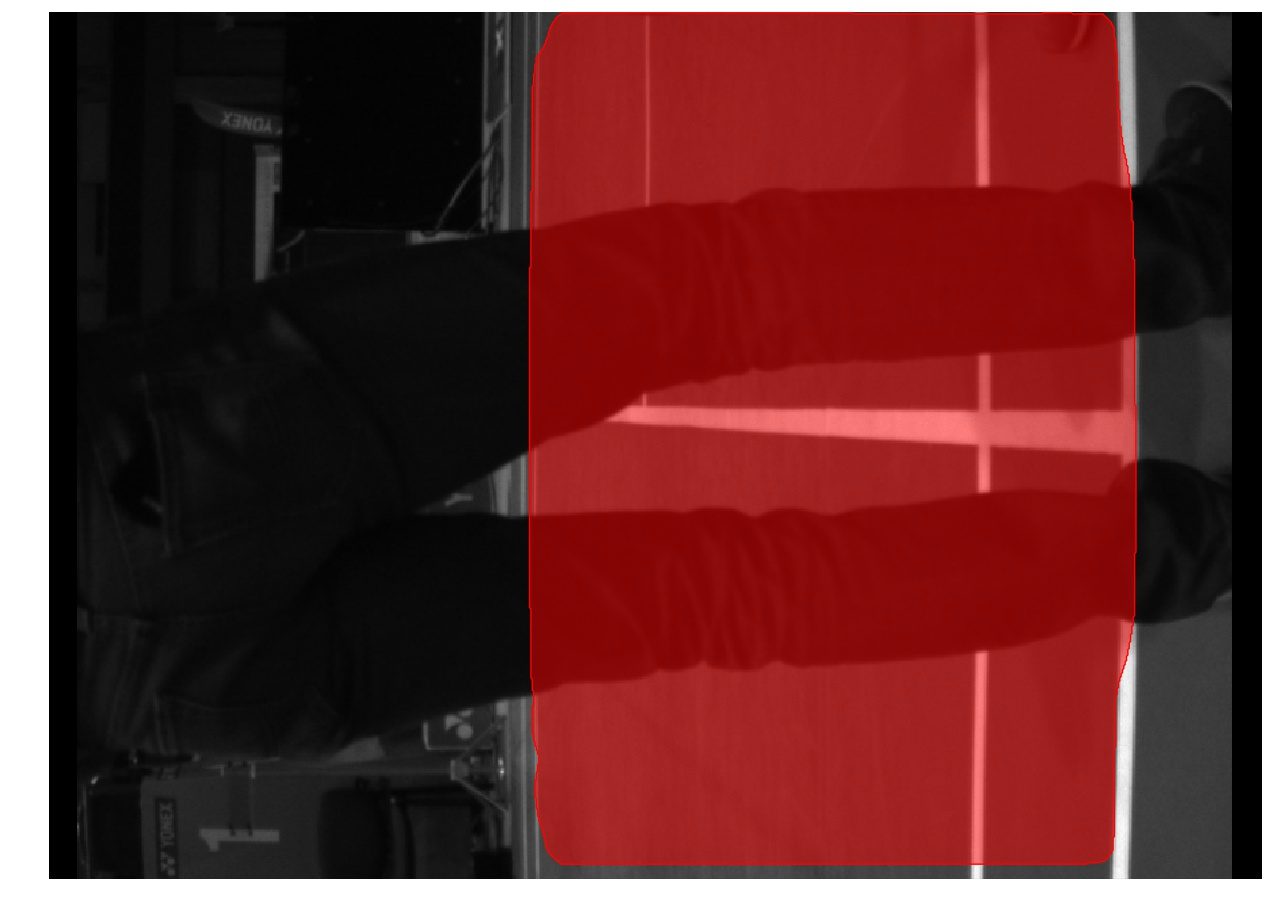
\includegraphics[width=\linewidth]{TP_frame_9.jpg}
    \caption{Przykładowy obraz z zaznaczonym obszarem zaklasyfikowanym jako~\textit{TP}}
    \label{fig:TP}
  \endminipage\hfill
  \minipage{0.45\textwidth}
    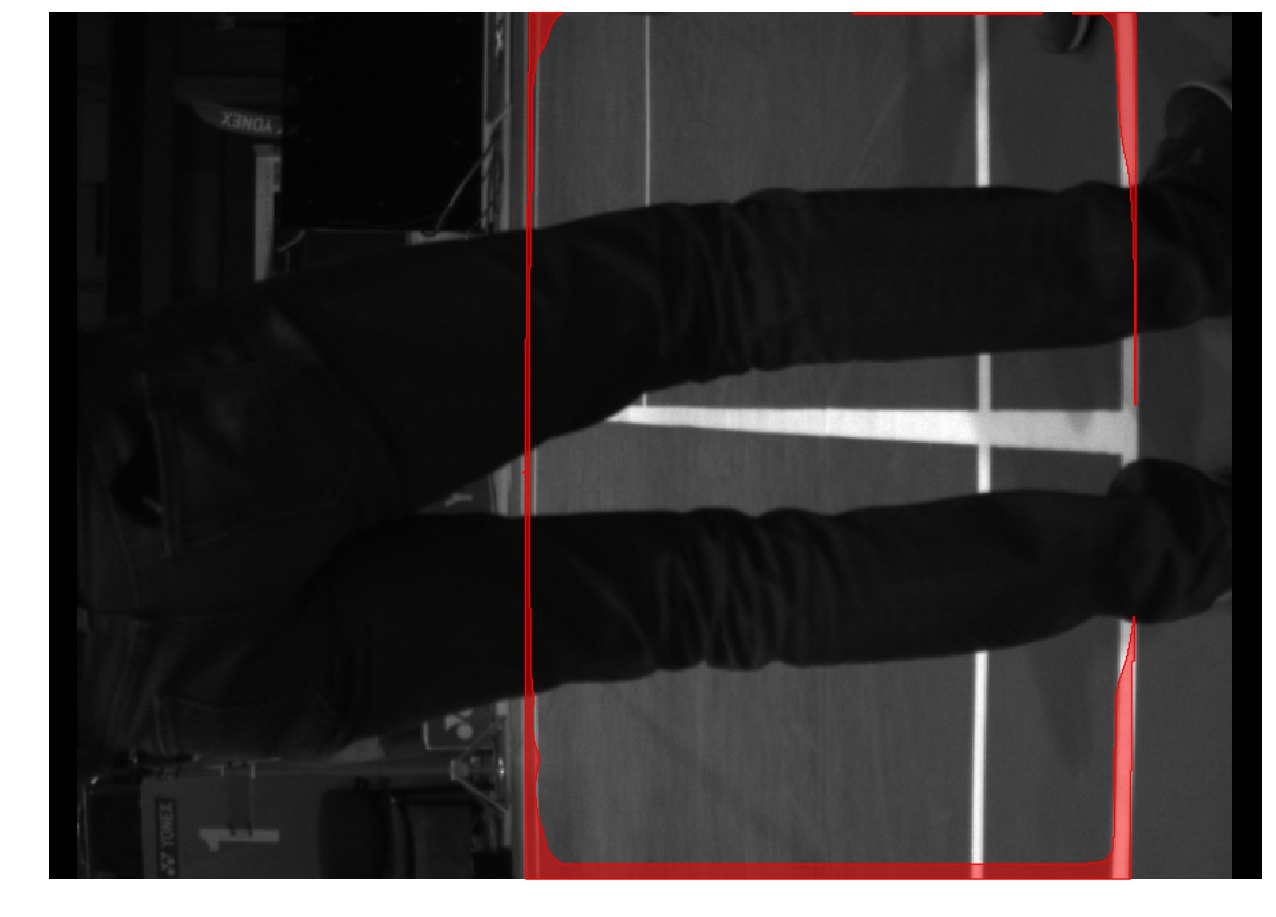
\includegraphics[width=\linewidth]{FN_frame_9.jpg}
    \caption{Przykładowy obraz z zaznaczonym obszarem zaklasyfikowanym jako~\textit{FN}}
    \label{fig:FN}
  \endminipage\hfill
  \vspace{0.5cm}
  \minipage{0.45\textwidth}
    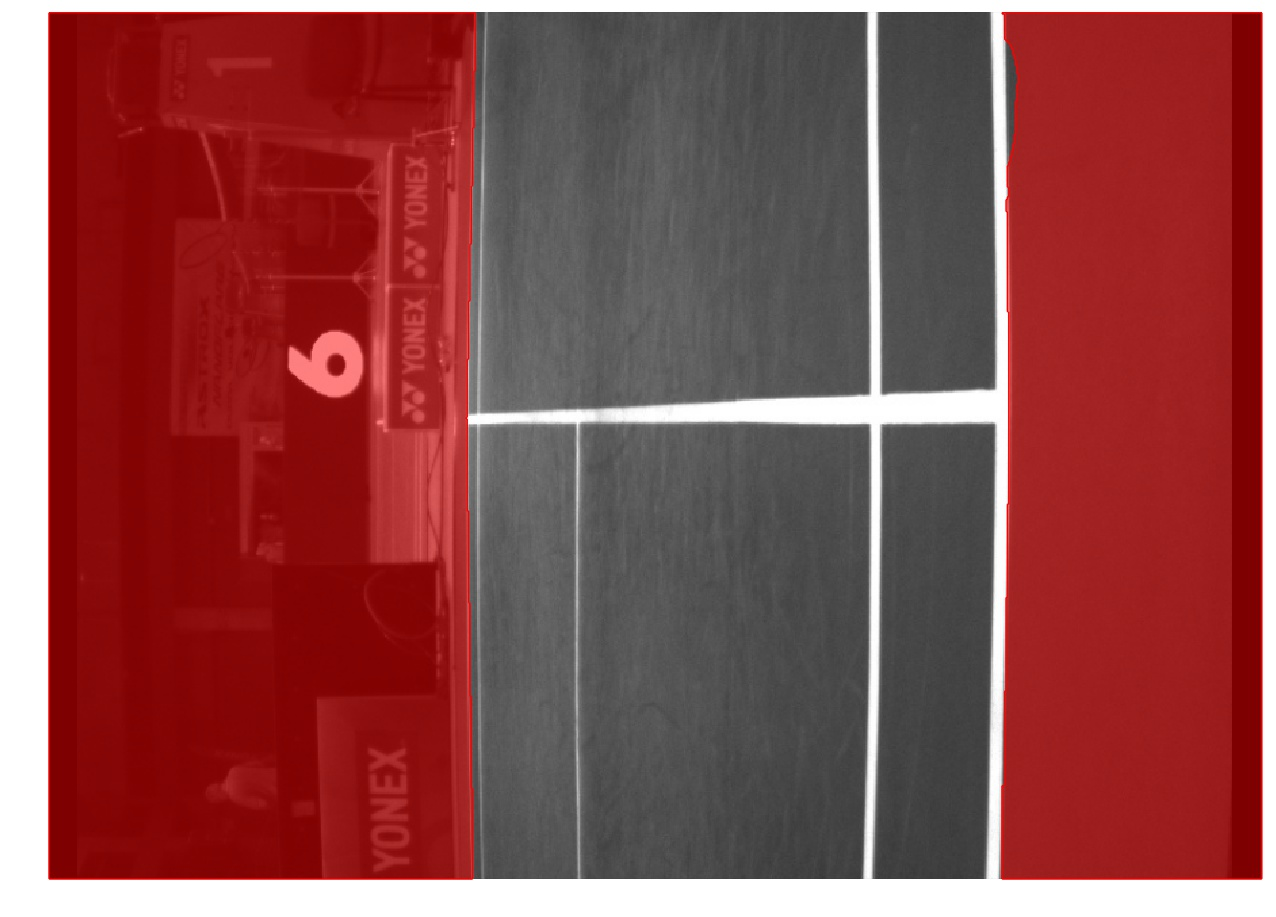
\includegraphics[width=\linewidth]{TN_frame_8.jpg}
    \caption{Przykładowy obraz z zaznaczonym obszarem zaklasyfikowanym jako~\textit{TN}}
    \label{fig:TN}
  \endminipage\hfill
  \minipage{0.45\textwidth}
    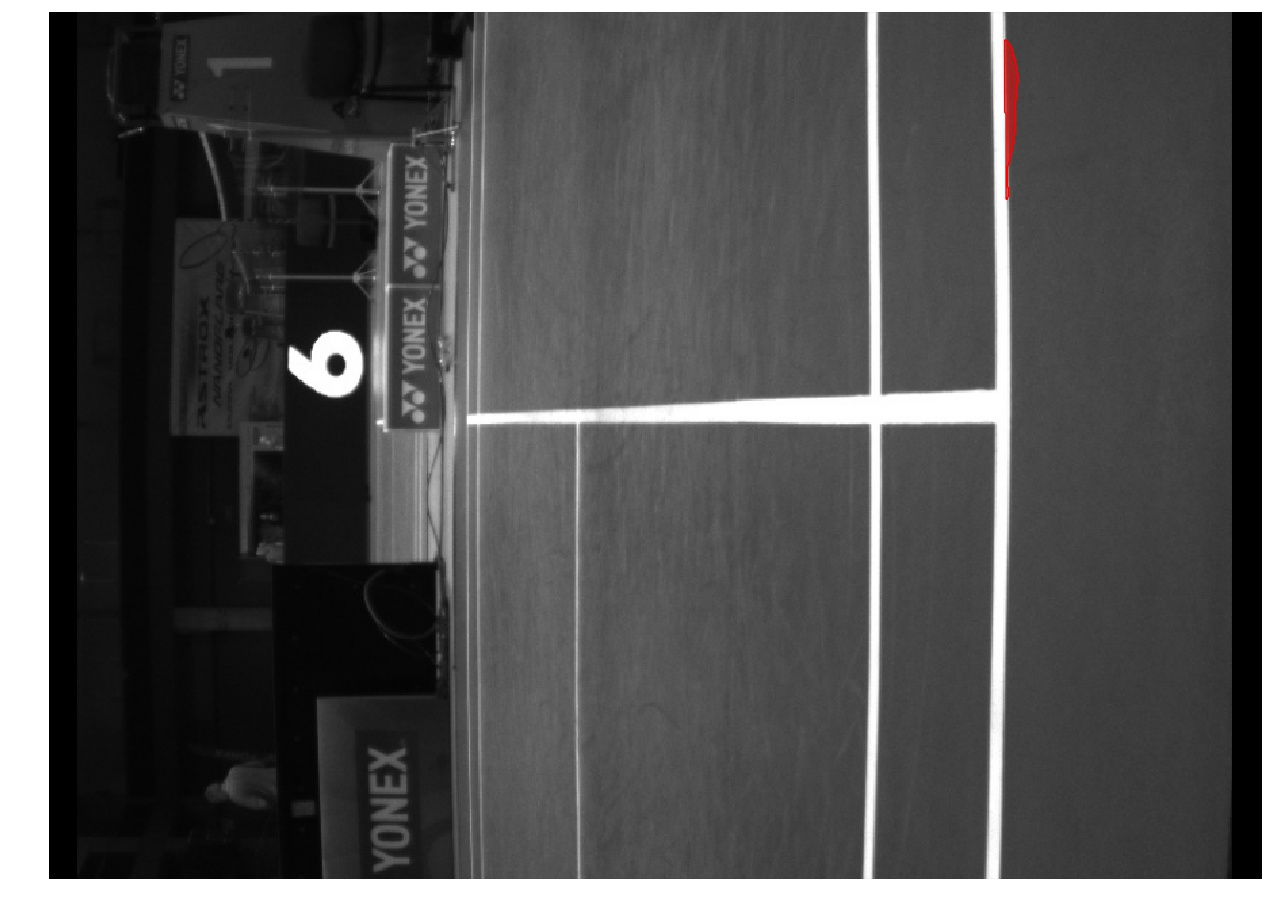
\includegraphics[width=\linewidth]{FP_frame_8.jpg}
    \caption{Przykładowy obraz z zaznaczonym obszarem zaklasyfikowanym jako~\textit{FP}}
    \label{fig:FP}
  \endminipage\hfill
\end{figure}
